%%%%%%%%%%%%%%%%%%%%%%%%%%%%%%%%%%%%%%%%%%%%%%%%%%%%%%%%%%%%%%%%%%%%%%%%%%%%%%%%%%
%%%%%%%%%%%%%%%%%%%%%%%%%%%%%%%%%%%%%%%%%%%%%%%%%%%%%%%%%%%%%%%%%%%%%%%%%%%%%%%%%%
\section{Results} \label{sec_res}
%%%%%%%%%%%%%%%%%%%%%%%%%%%%%%%%%%%%%%%%%%%%%%%%%%%%%%%%%%%%%%%%%%%%%%%%%%%%%%%%%%
%%%%%%%%%%%%%%%%%%%%%%%%%%%%%%%%%%%%%%%%%%%%%%%%%%%%%%%%%%%%%%%%%%%%%%%%%%%%%%%%%%

In this section, we present two series of results. First, Fourier analyses are 
carried out to analyze the performeance of the MIP-DSA acceleration scheme 
for an homogeneous infinite medium meshed with rectangular cells and discretized with PWLD.
The effects of the $S_n$ order and the cell aspect ratio on the spectral radius of the iterative 
scheme are also studied. Second, the MIP-DSA technique is implemented in a 2D \sn code that uses
arbitrary polygonal grids with a PWLD spatial discretization.  Numerical examples employ
several meshes: arbitrary quadrilaterals, arbitrary polygons, a regular layout of 
hexagons/triangles/rectangles, and a grid that mimics adaptive mesh refinement 
performed on rectangular cells. The MIP-DSA diffusion solves are performed using various
linear solvers: Conjugate Gradient (CG), Conjugate Gradient
Preconditioned with Symmetric Gauss-Seidel (PCG-SGS), Conjugate Gradient
Preconditioned with ML using Uncoupled aggregation (PCG-ML/U),
Conjugate Gradient Preconditioned with ML using MIS aggregation (PCG-ML/MIS),
and Conjugate Gradient Preconditioned AGMG (AGMG). 

%%%%%%%%%%%%%%%%%%%%%%%%%%%%%%%%%%%%%%%%%%%%%%%%%%%%%%%%%%%%%%%%%%%%%%%%%%%%%%%%%%
\subsection{Fourier Analyses}
%%%%%%%%%%%%%%%%%%%%%%%%%%%%%%%%%%%%%%%%%%%%%%%%%%%%%%%%%%%%%%%%%%%%%%%%%%%%%%%%%%

Fourier analyses are often performed to assess some of the properties of 
DSA-accelerated transport solves \cite{larsen_dsa,consistent_p1,more}. In a Fourier analysis,
the eigenvalues of the iteration matrix are analyzed, assuming a Fourier ansatz for the 
error modes \cite{}. For instance, the iteration matrices for the SI and SI+DSA schemes are given by
\begin{equation}
\bs{D L^{-1}M \Sigma} \quad \text{and} \quad \bs{I}-\bs{(I+A^{-1}\Sigma)(I-D L^{-1}M \Sigma)},
\end{equation}
respectively. The error modes are of the form $\exp(i \bs{\Lambda} \cdot \bs{r})$, with the
wave number $\bs{\Lambda}=[\lambda_x,\, \lambda_y]^T$. The expressions for these modes 
are inserted into the discretized equations and the spectral radius (largest eigenvalue in magnitude)
of the iteration matrices are sought for $0 \le \lambda_x \le 2\pi/X$ and $0 \le \lambda_y \le 2\pi/Y$,
where $X$, and $Y$ are the dimensions of the rectangular domain. The eigenvalues are obtained
using the {\tt eig} function of MATLAB and the search for the spectral radius is performed
using the Nelder-Mead simplex algorithm in MATLAB.


\subsubsection{Spectral radius as a function of the \sn order}
%%%%%%%%%%%%%%%%%%%%%%%%%%%%%%%%%%%%%%%%%%%%%%%%%%%%%%%%%%%%%%%%%%%%%%%%%%%%%%%%%%

This Fourier analysis is carried on a square cell ($X=Y$), using a
Gauss-Legendre-Chebyshev (GLC) angular quadrature. The medium is homogeneous with a 
scattering ratio $c=0.9999$; periodic boundary conditions are used. The results 
are plotted on \Cref{fig_fa_sn}, where the $x-$axis is the mesh size in mean free 
paths and the $y-$axis is the spectral radius. There are four curves corresponding 
to different $S_n$ orders: $S_2$, $S_4$, $S_8$ and $S_{16}$.
From \Cref{fig_fa_sn}, we conclude that MIP is stable for every 
cell size. The spectral radius is always less than 0.5, except for $S_2$ where 
it is about 0.7. In the fine mesh limit, the spatial continuum results are recovered:
the spectral radius of SI+DSA using an $S_2$ quadrature in 2D is $0.5c$; as the angular 
quadrature is refined, the standard result of $0.2247c$ for the spectral result is obtained.
\begin{figure}[!htbp]
  \centering
  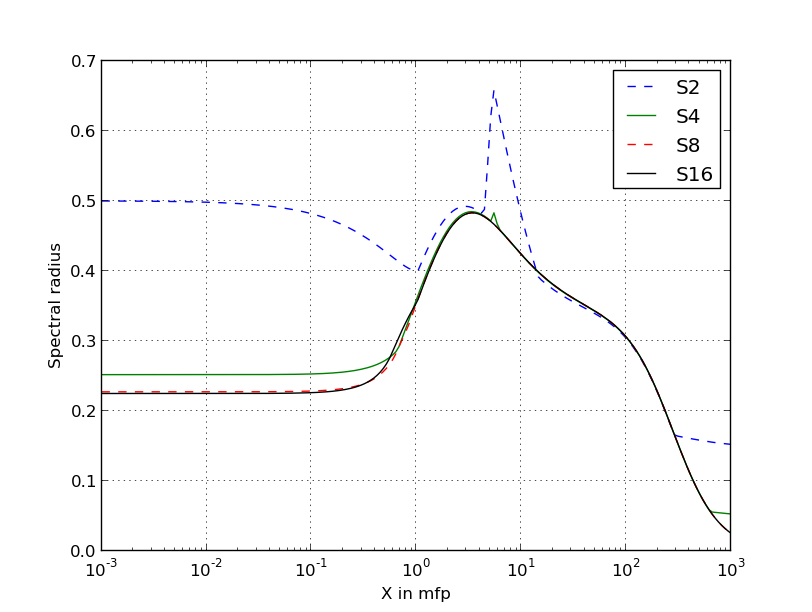
\includegraphics[width=0.7\textwidth]{sn_order_9999}
  \caption{Fourier analysis as a function of the mesh optical thickness, square cell,
    various \sn orders.}
  \label{fig_fa_sn}
\end{figure}

\subsubsection{Spectral radius as a function of the cell aspect ratio}
%%%%%%%%%%%%%%%%%%%%%%%%%%%%%%%%%%%%%%%%%%%%%%%%%%%%%%%%%%%%%%%%%%%%%%%%%%%%%%%%%%
For this Fourier analysis, we use a $S_{16}$ GLC quadrature. The medium is
again homogeneous with $c=0.9999$ and periodic boundary conditions apply. 
On \Cref{fig_fa_ar}, the five curves correspond to the following cell aspect 
ratios: $\frac{Y}{X}=\frac{1}{16}$, $\frac{Y}{X}=\frac{1}{4}$,
$\frac{Y}{X}=1$, $\frac{Y}{X}=4$, $\frac{Y}{X}=16$, and $\frac{Y}{X}=100$.
We note that the MIP-DSA scheme is stable for every aspect ratio tested, including 100, 
and that the maximum spectral radius shows little sensitivity the the aspect ratio.
\begin{figure}[!htbp]
  \centering
  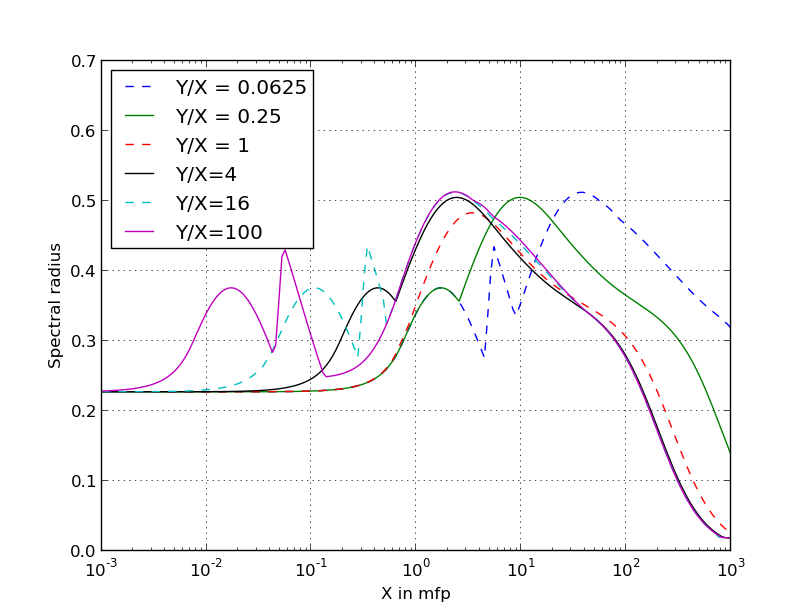
\includegraphics[width=0.7\textwidth]{aspect_ratio_9999_2}
  \caption{Fourier analysis as a function of the mesh optical thickness,
  $S_{16}$ angular quadrature, various aspect ratios.}
  \label{fig_fa_ar}
\end{figure}

%%%%%%%%%%%%%%%%%%%%%%%%%%%%%%%%%%%%%%%%%%%%%%%%%%%%%%%%%%%%%%%%%%%%%%%%%%%%%%%%%%
\subsection{Implementation of PWLD-discretized MIP-DSA in an $S_n$ code}
%%%%%%%%%%%%%%%%%%%%%%%%%%%%%%%%%%%%%%%%%%%%%%%%%%%%%%%%%%%%%%%%%%%%%%%%%%%%%%%%%%
The MIP-DSA scheme has been implemented in a 2D \sn code that employs a PWLD discretization
for arbitrary polygonal grids. Several test cases are presented.

\subsubsection{Homogeneous test problems}  \label{sec_homog}
%%%%%%%%%%%%%%%%%%%%%%%%%%%%%%%%%%%%%%%%%%%%%%%%%%%%%%%%%%%%%%%%%%%%%%%%%%%%%%%%%%

We compare the different linear solvers employed for MIP-DSA using a homogeneous medium, $100cm
\times 100cm$, $\Sigma_t = 1cm^{-1}$ and $\Sigma_s = 0.999cm^{-1}$, with
vacuum boundary conditions and a unit source of intensity $1cm^{-3}s^{-1}$. We
use an $S_8$ GLC angular quadrature, Source Iteration as solver
with relative tolerance of $10^{-8}$ and a relative tolerance of
$10^{-10}$ for MIP-DSA solver. The medium is discretized using two different meshes:
\begin{enumerate}
  \item a quadrilateral gridcomposed of 49236 quadrilateral
    cells (197,052 degrees of freedom); \textcolor{red}{$49236*4\ne 197052$!!!}
  \item a polygonal grid composed of 45,204 triangles, 823
    quadrilaterals, 4,978 pentagons, 4,155 hexagons, 725 heptagons, and 24
    octagons, for a total of 55,909 cells and 193,991 degrees of freedom. This
    example will allow us to test MIP and the different preconditioners on a
    mesh composed of different cell types.
\end{enumerate}
%
The meshes and the numerical solutions are given on \Cref{homog_test}.
In \Cref{comparison_homog_quad}, results obtained with the different linear solvers for MIP-DSA 
are compared for the quadrilateral grid.
In \Cref{comparison_homog_quad}, SI iterations is the number iterations of 
needed to solve the problem, Precond init is the time, in
seconds, needed to initialize the preconditioner used by CG, MIP calculation
is the total time, in seconds, spent solving DSA during the calculation, CG
iterations is the total number of CG iterations used to solve MIP, and Total
calculation is the time, in seconds, needed to solve the problem. 
We note that the accelerated transport solves only require 24 SI iterations, regardless of the linear solver
employed in MIP-DSA (as expected). Preconditioning CG significantly reduces the number of CG iterations.
%
We observe that algebraic multigrid processes, PGC-ML and AGMG, require 
about the same number of iterations (two orders of magnitude less than unpreconditioned CG). 
However, AMG is significantly faster than PCG-ML. We also note that PCG-SGS iteration is 
slower than one unpreconditioned CG iteration. Profiling of the code reveals that the
bottleneck is the function \emph{Ifpack\_PointRelaxation::ApplyInverseSGS\_FastCrsMatrix} 
of Trilinos. This function applies the forward and the backward substitutions required by SGS.
It is unclear why these substitutions are so costly. Also note that SGS is employed as
a pre- and post-smoother in the ML package of Trilinos and the same function
is once again the bottleneck of the method.
%
The different linear solvers are compared for the polygonal grid in \Cref{comparison_homog_poly}:
We note that using different spatial cell types in the same grid does not affect
the performance of MIP-DSA or that of its preconditioners.
%
\begin{figure}[!htbp]
  \centering
  \begin{subfigure}{0.75\textwidth}
    \centering
    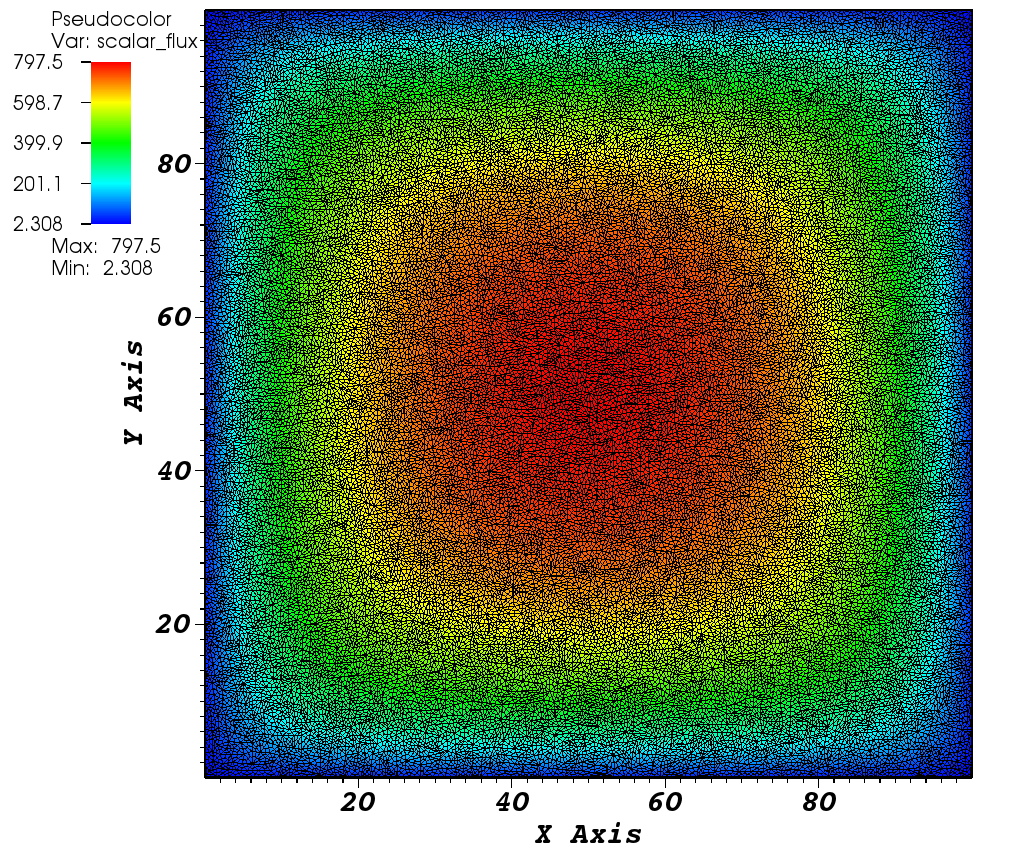
\includegraphics[width=\textwidth]{big_homog_quad_crop}
    \caption{Quadrilateral cells}
  \end{subfigure}
  \begin{subfigure}{0.75\textwidth}
    \centering
    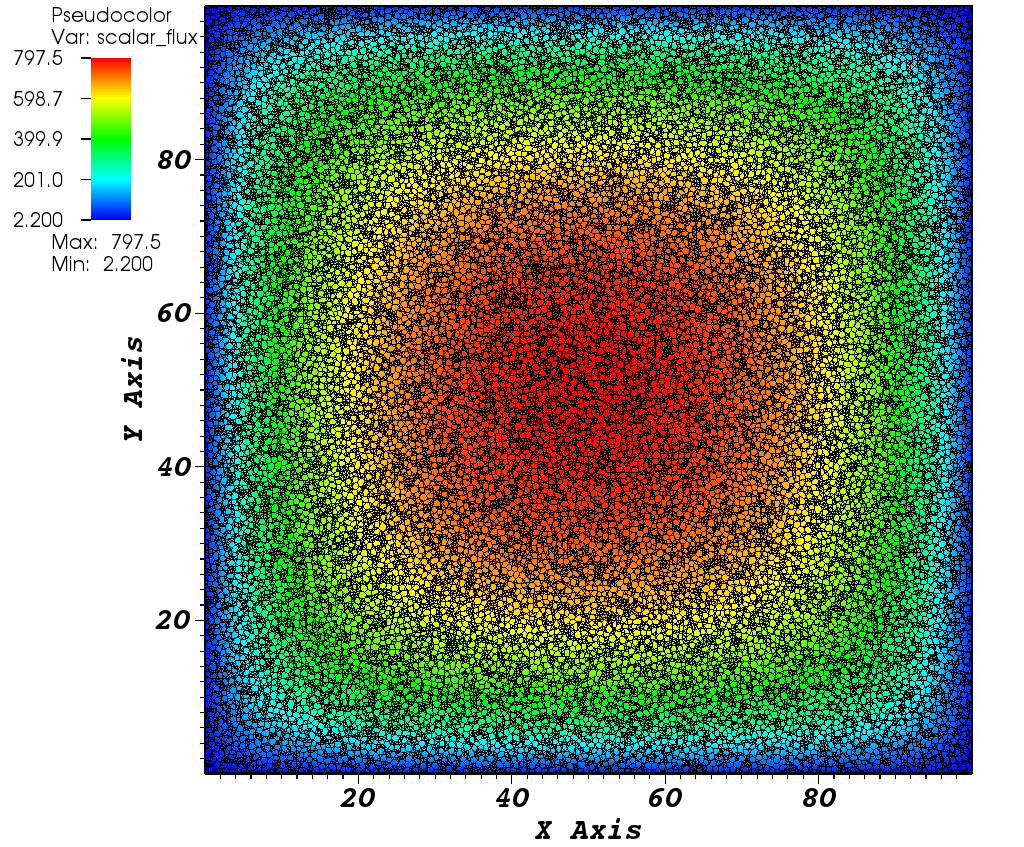
\includegraphics[width=\textwidth]{big_homog_poly_crop}
    \caption{Polygonal cells}
  \end{subfigure}
  \caption{Grids and scalar flux solutions for the homogenous material test problem}
  \label{homog_test}
\end{figure}
%
\textcolor{red}{what is the min value in the colorbar different for these grids??? The grids seem refined enough ....}
\begin{table}[!htbp]
  \begin{center}
    \caption{Comparison of different preconditioners for quadrilateral cells}
    \begin{tabular}{|c|c|c|c|c|c|c|}
      \hline
      & No-DSA & CG & PCG-SGS & PCG-ML/U & PCG-ML/MIS & AGMG \\
      \hline
      SI iterations   & 7311    & 24      & 24       & 24      & 24      & 24 \\
   Precond init (s)   & NA      & NA      & 0.171358 & 1.8255  & 9.56078 & 0.332 \\
MIP calculation (s)   & NA      & 1095.7  & 1311.76  & 192.622 & 197.632 & 29.9727 \\
      CG iterations   & NA      & 56649   & 17332    & 630     & 604     & 578 \\
Total calculation (s) & 39176.7 & 1264.98 & 1477.95  & 363.202 & 367.841 &
      194.568 \\
      \hline
    \end{tabular}
    \label{comparison_homog_quad}
  \end{center}
\end{table}
%
\begin{table}[!htbp]
  \begin{center}
    \caption{Comparison of different preconditioners for polygonal cells}
    \begin{tabular}{|c|c|c|c|c|c|c|}
      \hline
      & No-DSA & CG & PCG-SGS & PCG-ML/U & PCG-ML/MIS & AGMG \\
      \hline
      SI iterations   & 7311    & 23      & 23      & 23      & 23      & 23 \\
   Precond init (s)   & NA      & NA      & 0.06388 & 1.73379 & 8.0426  & 0.388 \\
MIP calculation (s)   & NA      & 877.861 & 1263.31 & 198.63  & 191.989 &
      31.242 \\
      CG iterations   & NA      & 46262   & 16712   & 652     & 603     & 555 \\
Total calculation (s) & 42666.7 & 1060.53 & 1447.53 & 382.275 & 384.422 &
      216.946 \\
      \hline
    \end{tabular}
    \label{comparison_homog_poly}
  \end{center}
\end{table}

\subsubsection{Heterogeneous medium}
%%%%%%%%%%%%%%%%%%%%%%%%%%%%%%%%%%%%%%%%%%%%%%%%%%%%%%%%%%%%%%%%%%%%%%%%%%%%%%%%%%

\textcolor{red}{why not make this problem thick? DSA is almost useless ....\\}

In this example, a heterogeneous geometry with three materials is used. It is 
composed of 184 triangles, 3,720 quadrilaterals and 2,791 regular hexagons of 
side $0.05cm$ for a total of 6,695 cells and 32,178 degrees of freedom (spatial 
unknowns per angular direction). The domain is $5.28275cm$ by $4.6cm$. 
Reflective boundary conditions are used. A $S_{16}$ GLC 
quadrature is used. The SI solver has a relative tolerance of 
$10^{-8}$ and the relative tolerance for MIP is $10^{-10}$. \Cref{hex_zones}
shows the problem geometry and the material properties are in given
\Cref{hex_prop}.
The different linear solvers for MIP-DSA are compared in \Cref{comparison_hex}.
%
\begin{figure}[!htbp]
  \centering
  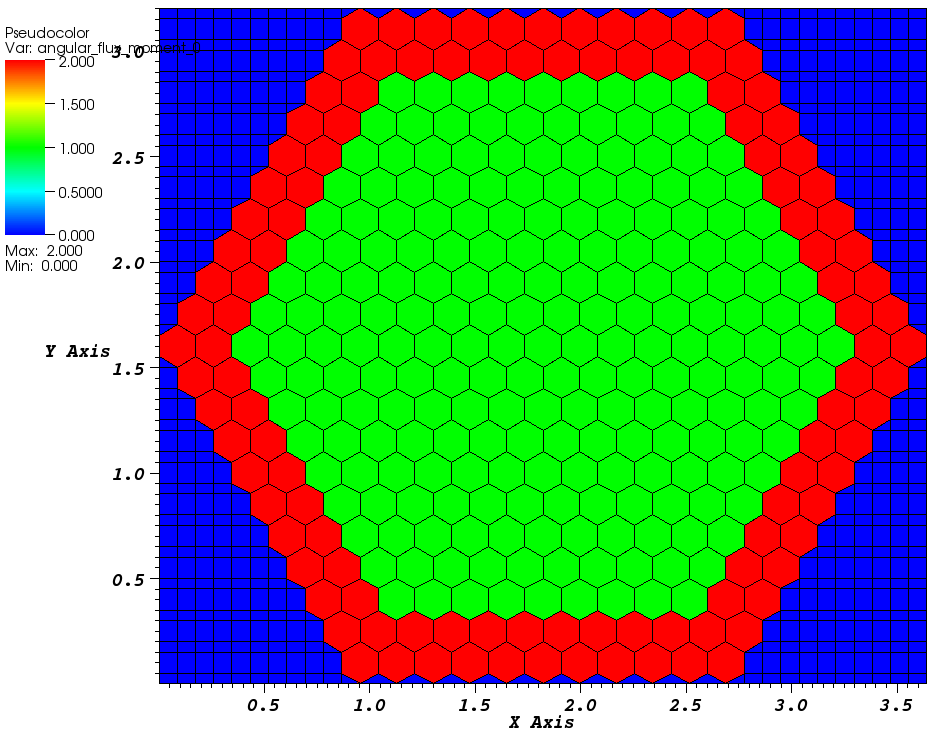
\includegraphics[width=0.6\textwidth]{source_crop}
  \caption{Material zones for the heterogeneous test problem}
  \label{hex_zones}
\end{figure}
%
\begin{table}[!htbp]
  \begin{center}
    \caption{Properties of the different zones}
    \begin{tabular}{|c|c|c|c|}
      \hline
       & Inner region & Intermediate region & Outer region \\
      $\Sigma_t$ $(cm^{-1})$ & 1.5 & 1.0 & 1.0 \\
      $\Sigma_s$ $(cm^{-1})$ & 1.4999 & 0.999 & 0.3 \\
     source $(cm^{-3}s^{-1}$ & 1.0 & 0.0 & 0.0 \\
      \hline
    \end{tabular}
    \label{hex_prop}
  \end{center}
\end{table}
%
%
\begin{table}[!htbp]
  \begin{center}
    \caption{Comparison of preconditioners, heterogeneous problem}
    \begin{tabular}{|c|c|c|c|c|c|c|}
      \hline
      & No-DSA & CG & PCG-SGS & PCG-ML/U & PCG-ML/MIS & AGMG\\
      \hline
      SI iterations & 278     & 17      & 17        & 17       & 17      & 17  \\
   Precond init (s) & NA      & NA      & 0.0160661 & 0.368768 & 1.41632 &
      0.07  \\
MIP calculation (s) & NA      & 58.422  & 126.93    & 33.2225  & 31.3045 &
      2.924 \\
      CG iterations & NA      & 12214   & 6679      & 415      & 386     & 248  \\
Total calculation (s) & 910.566 & 120.889 & 190.413 & 99.7524  & 97.4666 &
      70.6424 \\      
      \hline
    \end{tabular}
    \label{comparison_hex}
  \end{center}
\end{table}
%
The remarks made in \Cref{sec_homog} for the homogeneous test problem
remain mostly unchanged. MIP-DSA is effective for this heterogeneous test case and AGMG is
still the fastest solver. It is interesting to note that, contrary to the
homogeneous tests where the number of CG iterations remained similar for all
algebraic multigrid preconditioners, in this test, AGMG requires
significantly fewer iterations than the Trilinos implementations, PCG-ML/U and and PCG-ML/MIS.

\subsubsection{Locally refined grid}
%%%%%%%%%%%%%%%%%%%%%%%%%%%%%%%%%%%%%%%%%%%%%%%%%%%%%%%%%%%%%%%%%%%%%%%%%%%%%%%%%%

%\cite{mip}
In this example, a domain of $10cm\times 10cm$ is used. The left and bottom
boundaries are reflective whereas the right and the top boundaries are vacuum. 
\Cref{zone_amr} shows the material zoning and the mesh used. Material properties 
are given in \Cref{prop_amr}. The grid used mimics meshes obtained via adaptive mesh
refinement: the cells at the interfaces between two material are refined once more.
There are 10,720 cells: 10,482 quadrilaterals, 236 pentagons,
and 2 hexagons for a total of 43120 degrees of freedom. 
%
The distribution of cells is given \Cref{fig_pol_dist}.
A $S_{16}$ GLC quadrature is employed. The tolerance on SI is $10^{-8}$ and
the tolerance on the CG solvers is $10^{-10}$.
The different linear solvers for MIP-DSA are compared in \Cref{table_amr}.
%
The conclusions are similar to the ones made for our previous tests.
%
\begin{figure}[!htbp]
  \centering
  \begin{subfigure}{0.75\textwidth}
    \centering
    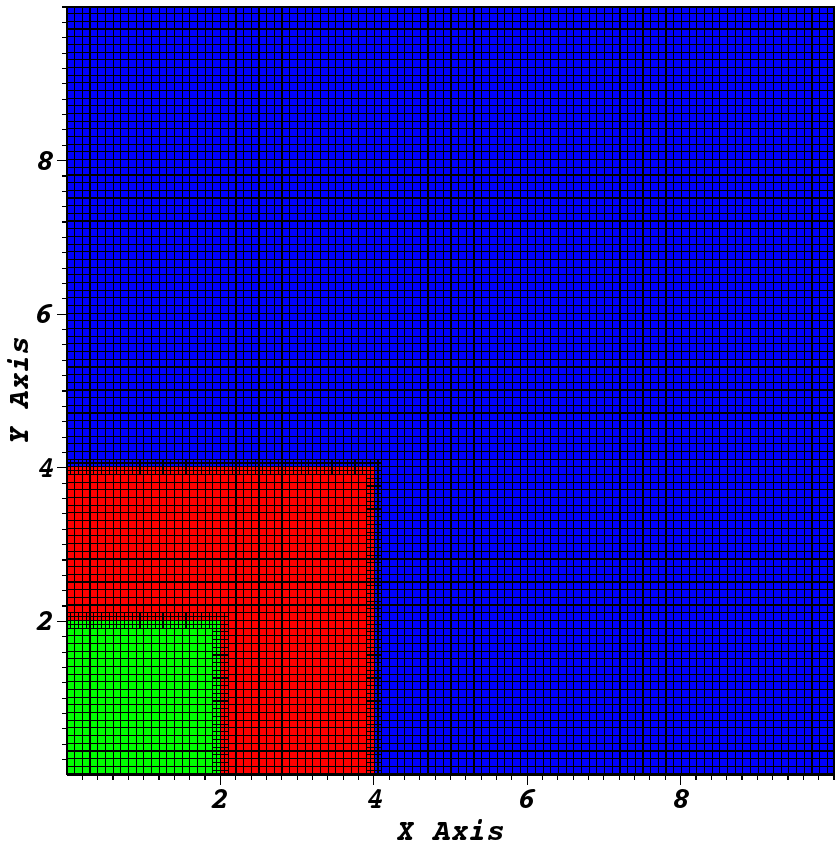
\includegraphics[width=6cm]{zone_amr}
    \caption{Material regions}
  \end{subfigure}
  \begin{subfigure}{0.75\textwidth}
    \centering
    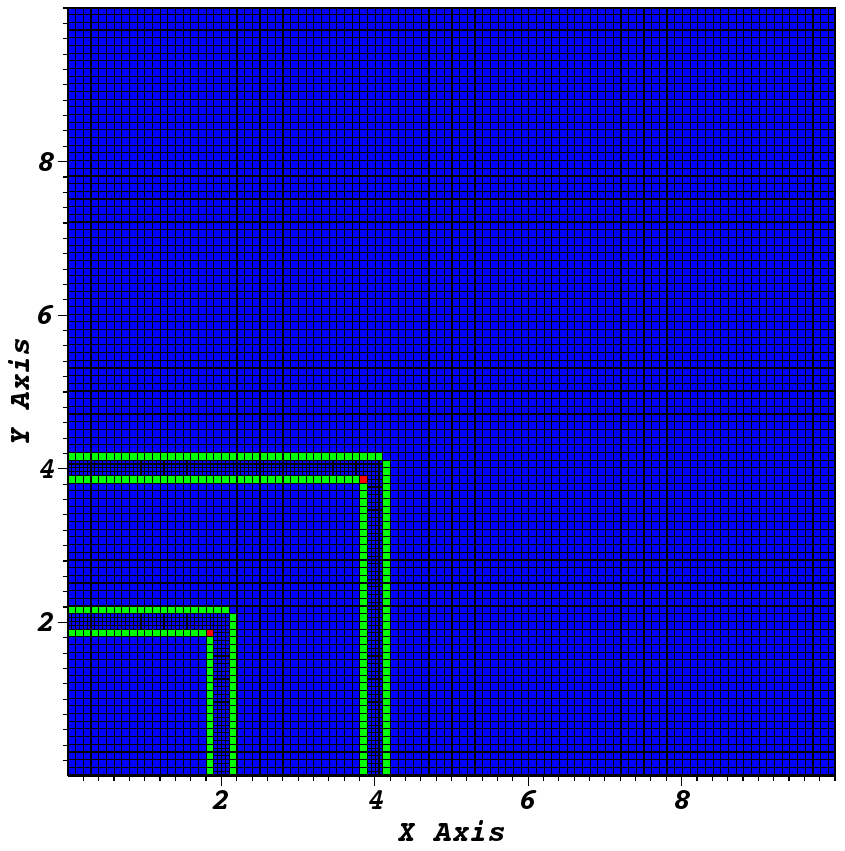
\includegraphics[width=6cm]{polygon_amr}
    \caption{Polygons distribution (the blue cells are quadrilaterals, the green cells are pentagons, and the red cells are hexagons)}
    \label{fig_pol_dist}
  \end{subfigure}
  \caption{AMR-like test domain}
  \label{zone_amr}
\end{figure}
%
\begin{table}
  \begin{center}
    \caption{Material properties, AMR-like test problem}
    \begin{tabular}{|c|c|c|c|}
      \hline
      & Inner region & Intermediate region & Outer region  \\ \hline
    $\Sigma_t$ $(cm^{-1})$ & 1.5  & 1.  & \textcolor{red}{1.0 ?} \\
    $\Sigma_s$ $(cm^{-1})$ & 1.44 & 0.9 & 0.3 \\
  Source $(cm^{-3}s^{-1})$ & 1.0  & 0.0 & 0.0 \\
      \hline
    \end{tabular}
    \label{prop_amr}
  \end{center}
\end{table}
%
%where the blue cells are quadrilaterals, the green cells are pentagons, and
%the red cells are hexagons. This mesh is typical of a mesh obtained after one 
%level of adaptive mesh
%refinement (the cells at the interface of different materials have been refined
%once). We see that instead of introducing hanging nodes, we have introduce
%pentagons and hexagons in the mesh.
\begin{table}[H]
  \caption{Comparison of preconditioners on AMR mesh}
  \begin{center}
    \begin{tabular}{|c|c|c|c|c|c|c|}
      \hline
       & No-DSA & CG & PCG-SGS & PCG-ML/U & PCG-ML/MIS & AGMG \\
      \hline
   SI iterations & 184     & 19      & 19       & 19      & 19       & 19 \\
Precond init (s) & NA      & NA      & 0.043463 & 0.358002 & 1.19301 & 0.0111\\
MIP calculation (s) & NA   & 48.1908 & 81.0992  & 25.2699 & 25.0699  & 
      2.56198\\
   CG iterations & NA      & 11300   & 4734     & 361     & 361      & 264 \\
     Total calculation (s) & 802.985 & 138.825 & 172.423  & 116.018 & 116.517  &
      94.1963\\
      \hline
    \end{tabular}
    \label{table_amr}
  \end{center}
\end{table}

\subsubsection{High aspect ratio grid}
%%%%%%%%%%%%%%%%%%%%%%%%%%%%%%%%%%%%%%%%%%%%%%%%%%%%%%%%%%%%%%%%%%%%%%%%%%%%%%%%%%

For the next two examples, the domain is square $100cm
\times 100cm$ with vacuum boundaries. There are 10000 cells and thus, 40000
degrees of freedom. The relative tolerance on SI is $10^{-8}$ and the relative
tolerance for CG is $10^{-10}$. We use a $S_8$ GLC quadrature, $\Sigma_t =
1cm^{-1}$, and $\Sigma_s = 0.999cm^{-1}$. The source is $1n/(cm^3s)$. In the
first test, the domain is discretized by 100 cells along $x$ and 100 cells
along $y$, i.e., square cells with aspect ratio of one. In the second run, 
the domain is discretized by 1000 cells along $x$ and 10 cells along $y$ 
(the aspect ratio is 100).
%
As expected, solving the MIP-DSA equations requires more CG iterations when the aspect
ratio increases. PCG-ML/U and PCG-ML/MIS are significantly more affected by the
increase in the aspect ratio than the other methods. AGMG is the least
affected by the change of aspect ratio and is the best performing
preconditioner.
%
\begin{table}[!htbp]
  \caption{Comparison of preconditioners on rectangular grid with an aspect
  ratio of 1}
  \begin{center}
    \begin{tabular}{|c|c|c|c|c|c|c|}
      \hline
       & No-DSA & CG & PCG-SGS & PCG-ML/U & PCG-ML/MIS & AGMG \\
      \hline
      SI iterations & 7311      & 21      & 21      & 21       & 21      & 21 \\
   Precond init (s) & NA        & NA      & 0.01422 & 0.051373 & 1.13144 &
      0.044 \\
MIP calculation (s) & NA        & 32.3825 & 73.8422 & 24.0707  & 25.0065 &
      1.7114 \\
      CG iterations & NA        & 8363    & 4853    & 376      & 375     &
      221\\
Total calculation (s) & 7356.96 & 56.8993 & 98.2609 & 50.1247  & 51.5396 &
      25.9306 \\
      \hline
    \end{tabular}
    \label{table_ar_1}
  \end{center}
\end{table}
%
\begin{table}[!htbp]
  \caption{Comparison of preconditioners on rectangular grid with an aspect
  ratio of 100}
  \begin{center}
    \begin{tabular}{|c|c|c|c|c|c|c|}
      \hline
       & No-DSA & CG & PCG-SGS & PCG-ML/U & PCG-ML/MIS & AGMG \\
      \hline
      SI iterations & 7304    & 24      & 24        & 24       & 24      & 24 \\
   Precond init (s) & NA      & NA      & 0.0164239 & 0.362463 & 1.03128 & 0.052 \\
MIP calculation (s) & NA      & 372.227 & 742.902   & 941.06   & 922.258 &
      6.93176 \\
      CG iterations & NA      & 84802   & 43466     & 14180    & 13896   & 821 \\
Total calculation (s) & 9035.6 & 414.301 & 784.77   & 985.796  & 966.77  &
      44.7032 \\
      \hline
    \end{tabular}
    \label{table_ar_100}
  \end{center}
\end{table}                  
